\usetikzlibrary{arrows.meta}
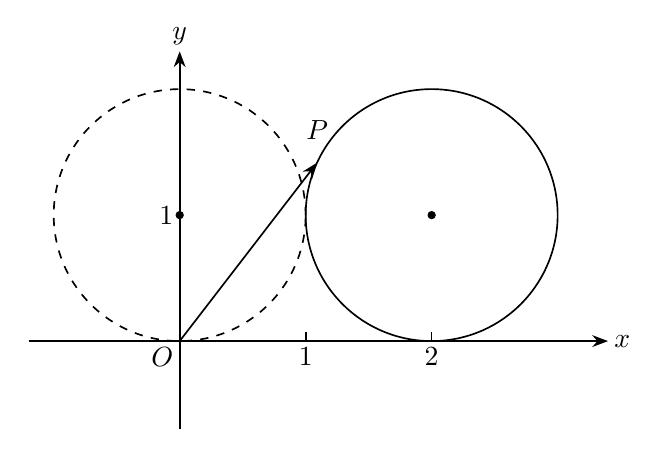
\begin{tikzpicture}[x=1.6cm,y=1.6cm,line width=.6pt,font=\normalsize,every node/.style={inner sep=0pt},>=Stealth]
\draw[->] (-1.2,0) -- (3.4,0) node[right,inner sep=0pt,xshift=2pt] {$x$};
\draw[->] (0,-0.7) -- (0,2.3) node[above,inner sep=0pt,yshift=2pt] {$y$};
\node[below left,inner sep=0pt,xshift=-2pt,yshift=-2pt] at (0,0) {$O$};
\draw (1,0) -- (1,0.07);
\node[below,inner sep=0pt,yshift=-2pt] at (1,0) {$1$};
\draw (2,0) -- (2,0.07);
\node[below,inner sep=0pt,yshift=-2pt] at (2,0) {$2$};
\draw[dashed] (0,1) circle[radius=1];
\draw (2,1) circle[radius=1];
\fill (0,1) circle(1.5pt);
\fill (2,1) circle(1.5pt);
\node[left,inner sep=0pt,xshift=-2pt] at (0,1) {$1$};
\coordinate (P) at (1.090702573174,1.416146836547);
\draw[->] (0,0) -- (P);
\node[above,inner sep=0pt,yshift=8pt] at (P) {$P$};
\end{tikzpicture}
